%%
%% Dibujos
%%
%\usepackage{tikz}
\usetikzlibrary{shapes,shapes.geometric,arrows,calc,fit,shadows,positioning,decorations.markings}
\tikzstyle{oval} = [ellipse, top color=white!70!Green!70, bottom color=Green, node distance=2cm, minimum height=2em, draw=Green]
\tikzstyle{arrow} = [->, decoration={markings,mark=at position 1 with {\arrow[scale=2]{>}}},
    postaction={decorate},
    shorten >=0.4pt]
\tikzstyle{marco} = [top color=white!70!AzulCielo!70, bottom color=AzulCielo, draw=AzulCielo]

% We need layers to draw the block diagram
\pgfdeclarelayer{background}
\pgfdeclarelayer{foreground}
\pgfsetlayers{background,main,foreground}


%opening
%\title{Marcos}
%\author{Inteligencia Artificial}

%\begin{document}

%\maketitle

\section{Marcos (Frames)}

El sistema de Marcos en la base de la programación Orientada a Objetos actual, por lo que los conceptos aquí citados resultarán familiares.  Sin embargo, la teoría de marcos cubre casos que la mayoría de los lenguades de programación populares evitan, especialmente la herencia múltiple.  Además, el término \textit{marco} en general puede referirse tanto a una instancia como a una clase \cite{Winston}.

Dos notaciones comunes para representar a los marcos son:
\begin{lstlisting}
 (nombre ranura(valor-de-ranura) ranura-1(valor-de-ranura-1)...)
\end{lstlisting}

\begin{figure}[H]
\centering
\begin{tikzpicture}
 \node (name) {Nombre};
 \node [label=west:slot, draw, below of=name, anchor=south west] (slot) {valor-de-ranura};
 \begin{pgfonlayer}{background}
  \node [marco, fit=(name)(slot), draw, inner sep=5pt, align=left] (marco) {};
 \end{pgfonlayer}
\end{tikzpicture}
\caption{Diagrama de un marco.}
\end{figure}

Los marcos se originaron a partir de las redes semánticas.  Una \textbf{red semántica} está compuesta por nodos y ligas entre ellos.  Cada liga lleva por nombre el tipo de relación entre los nodos vinculados.  Para reinterpretar una red semántica como un sistema de marcos se considera a cada nodo con las ligas vinculadas a él.

\begin{figure}[H]
\centering
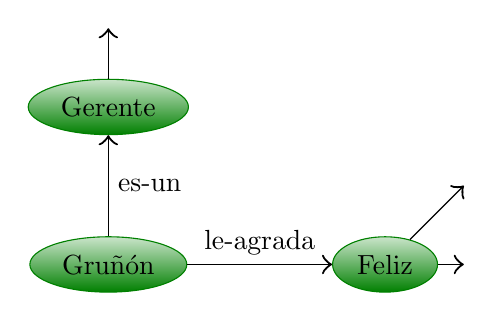
\begin{tikzpicture}
 \node [oval] (manager) {Gerente};
 \node [oval, below of=manager] (grumpy) {Gruñón};
 \node [oval, right of=grumpy, node distance=10em] (happy) {Feliz};
 \draw [arrow] (grumpy) -- node [above] {le-agrada} (happy);
 \draw [arrow] (grumpy) -- node [right] {es-un} (manager);
 \draw [arrow] (manager) -- ($(manager) + (0,+1)$);
 \draw [arrow] (happy) -- ($(happy) + (+1,0)$);
 \draw [arrow] (happy) -- ($(happy) + (+1,+1)$);
\end{tikzpicture}
\\ \vspace{5mm}
\begin{tikzpicture}
 \node (name) {Gerentes};
 \node [label=west:, draw, below of=name, anchor=south west, text width=4em] (slot) {};
 \begin{pgfonlayer}{background}
  \node [marco, fit=(name)(slot), inner sep=5pt, align=left] (marco) {};
 \end{pgfonlayer}

 \node [below of=name, node distance=7em] (grumpy) {Gruñón};
 \node [label=west:is-a, draw, below of=grumpy, anchor=south west, text width=4em] (gEs_un) {};
 \node [label=west:le-agrada, draw, below of=gEs_un, anchor=south west, text width=4em] (gLikes) {Feliz};
 \begin{pgfonlayer}{background}
  \node [marco, fit=(grumpy)(gEs_un)(gLikes), draw, inner sep=5pt, align=left] (marco1) {};
 \end{pgfonlayer}
 \draw [*->] (gEs_un.center) -- +(0,1.7) -- +(-2.8,1.7) -- +(-2.8,2.7) -- (manager.west);

 \node [right of=grumpy, node distance=10em] (happy) {Feliz};
 \node [label=west:, draw, below of=happy, anchor=south west, text width=4em] (hEs_un) {};
 \node [label=west:, draw, below of=hEs_un, anchor=south west, text width=4em] (hLikes) {};
 \begin{pgfonlayer}{background}
  \node [marco, fit=(happy)(hEs_un)(hLikes), draw, inner sep=5pt, align=left] (marco2) {};
 \end{pgfonlayer}
\end{tikzpicture}
\caption{Arriba: red semántica.  Abajo: diagrama de un marco; es posible usar ligas o nombres de otros marcos para llenar las ranuras.}
\end{figure}

Hay dos clases de marcos:
\begin{itemize}
 \item Clases. a.k.o. = \emph{a kind of} <class>
 \item Ejemplares (o instancias). is-a <class>
\end{itemize}

\subsection{Procedimientos de acceso}
\begin{description}
 \item[Durante-la-construcción] construye marcos instancia.  Puede asignar valores por defecto a las ranuras mediante los \textbf{procedimientos-de-construcción} sugeridos por las clases y superclases de la instancia, de acuerdo con la \textbf{lista-de-precedencia}.
 \item[Durante-la-escritura] Asigna valores a las rendijas.  Ayudan a mantener restricciones entre ranuras relacionadas.  Por ejemplo: si en la ranura \textit{constitución-física} se escribe \textit{delgado}, escribir \textit{pequeño} en la ranura \textit{apetito}.
 \item[Durante-la-lectura] Devuelve los valores de las rendijas.
 \item[Cuando-se-solicite] Sobrecargan los valores por defecto heredados.  Pueden utilzar valores de otras ranuras que fueron llenadas durante la construcción de la instancia.
 \item[Con-respecto-a] reciben como argumento el contexto en el que la propiedad debe ser evaluada.  Por ejemplo, si se pide la estatura del enano Blimpy con repecto a un duente, el valor es \textit{grande}.  Si se pide su estatura con respecto a un enano promedio, tal vez el valor se \textit{pequeño}.
 \item[Cuando-aplica] semejante a los procedimientos \textit{con-respecto-a}, pero para acciones.  Calculan el mecanismo adecuado para cada acción dependiendo del contexto.  Por ejemplo: \texttt{comer(sopa)} utiliza una cuchara, mientras que \texttt{comer(ensalda)} require un tenedor.
\end{description}

\subsection{Lista de precedencia}
Hay dos criterios útiles para la obtención de una lista de precedencia:
\begin{enumerate}
 \item Cada clase debe aparecer en la lista de precedencia antes que cualquiera de sus superclases.
 \item Cada superclase directa de una clase dada debe aparecer en la lista de precedencia antes que cualquier superclase directa que se encuentre a su derecha.
\end{enumerate}

Si el tipo de herencia es simple, basta con recorrer la gráfica de marco primero en profundidad.  Si la herencia es múltiple, pero no se forman rombos en la jerarquía, basta con agregar la regla \textbf{up-to-join-proviso}.  Esta regla indica que, cada superclase que sea visitada más de una vez durante el recorrido primero en profundidad, de izquierda a derecha, debe ser ignorada hasta que la clase se encontrada por última vez.  Sin embargo, para el caso general, es necesario aplicar el algoritmo \textbf{ordenamiento topológico} [\pref{alg:topological_sort}].

% \begin{algorithm}[htp!]
%  \caption{Ordenamiento topológico.}\label{alg:astar}
% \begin{algorithmic}
%  \State listaMarcos $\leftarrow$ Crear una lista de todos los marcos accesibles desde el nodo instancia a través de relaciones is-a y a.k.o, incluyendo al nodo instancia.
%  \ForAll{marco \textbf{in} listaMarcos}
%    \If{marco.is-a $\neq\emptyset$}
%      \State listaRestricciones.add(marco, marco.is-a[0])
%      \ForAll{i,clase \textbf{in} marco.is-a[1:-1]}
%       \State listaRestricciones.add(clase, marco.is-a[i+1])
%      \EndFor
%    \EndIf
%    \If{marco.ako $\neq\emptyset$}
%      \State listaRestricciones.add(marco, clase.ako[0])
%      \ForAll{i,clase \textbf{in} clase.ako[1:-1]}
%       \State listaRestricciones.add(clase, clase.ako[i+1])
%      \EndFor
%    \EndIf
%  \EndFor
%  \ForAll{pair in listaRestricciones}
%   \If{pair.left \notin }
%  \EndFor
% \end{algorithmic}
% \end{algorithm}

\begin{algorithm}[H]
 \caption{Ordenamiento topológico.}\label{alg:topological_sort}
\begin{algorithmic}
 \State listaMarcos $\leftarrow$ Crear una lista de todos los marcos accesibles desde el nodo instancia a través de relaciones is-a y a.k.o, incluyendo al nodo instancia.
 \ForAll{marco \textbf{in} listaMarcos}
  \State listaRestricciones.añadir(marco, primer clase a la izquierda)
  \State Añadir listaRestricciones cada par clase-clase de izquierda a derecha
  \State Si el marco no tiene clases o superclases añadirlo solo.  Un elemento solo cuenta como estar a la izquierda del par.
 \EndFor
 \Repeat
 \State Tomar al marco que aparezca a la izquierda de al menos un par, pero a la deracha de ninguno.
  \If{Hay más de un marco sólo a la izquierda}
   \State Recorrer la listaDePresedencia desde el final hacia el inicio.
   \State Seleccionar el marco que sea clase o superclase directa del elemento más cercano al final de la listaDePresedencia.
  \EndIf
  \State Añadirlo a listaDePresedencia
  \State Eliminar a todos los pares donde aparezca.
 \Until{listaRestricciones $=\emptyset$}
\end{algorithmic}
\end{algorithm}

\begin{figure}
 \centering
 %\includegraphics[width=\textwidth]{../Figuras/Marcos.png}
  \caption{Objetos y relaciones diversas entre ellos.  Particularmente: \emph{un-tipo-de}, \emph{es-un} que permiten heredar comportamientos.}
\end{figure}


\subsection{Aplicaciones}
Extracción de información de textos en un contexto definido, así como producción de textos a partir de instancias con información.
Almacenamiento de información para sistemas expertos como:
\begin{itemize}
 \item CYC (\hurl{http://www.cyc.com/} y \hurl{http://www.cyc.com/platform/opencyc})
 \item OpenMind Common Sense \hurl{http://commons.media.mit.edu/}
\end{itemize}

Existe también una base datos del idioma Inglés donde las palabras están relacionadas unas con otras:
\begin{itemize}
 \item WordNet \hurl{http://wordnet.princeton.edu/}
\end{itemize}
 
%\end{document}
